\documentclass[letterpaper,10pt]{article}

\usepackage{template}
\usepackage{indentfirst}
\usepackage{listings}


\begin{document}

\begin{tabular}{ccl}
\begin{tabular}{c}

\psfig{file=puclogo.eps}
\end{tabular}
\begin{tabular}{l}
\tiny{\ }\\ \normalsize
\sc Pontificia Universidad Católica de Chile\\
\sc Escuela de Ingeniería\\
\sc Departamento de Ingeniería Industrial y de Sistemas\\
\sc ICS3105 Optimización Dinámica (2018-2)\\
\sc Profesor Mathias Klapp
\end{tabular}
\end{tabular}
\begin{center}
\LARGE \bf Tarea 2\\
\vspace{1ex}\small Ignacio Guridi (iguridi@uc.cl) - Raimundo Herrera (rjherrera@uc.cl)
\end{center}

\section{}

\begin{enumerate}
    \item Para este problema la modelación es muy similar a la del Secretary Problem. El problema visto como un MDP es el siguiente:
    
    \begin{itemize}
        \item Etapas: $\{1, \dots, n\}$ con $n$ el número de lotes de estacionamiento
        \item Estado: 1 si es la mejor posibilidad de estacionamiento hasta ahora 0 si no. Esto se traduce en que será la mejor posibilidad si está vacío o no. 1 lote vacío, 0 lote lleno.
        \item Decisión: 1 si me estaciono, 0 si no.
        \item Valor inmediato: 
        \[
        r_t(s, x) = 
            \begin{cases}
                r_t(0,0) = r_t(0, 1) = r_t(1, 0) = 0\\
                r_t(1,1) = t\\
            \end{cases}
        \]
        \item Probabilidades: como solo depende de si el estacionamiento está vacío o no, se colapsa desde $p_t(s'\mid_{s,x})$ a $p_t(s')$
        \[
        p_t(s') = 
            \begin{cases}
                p_t(0) = 1 - p_t\\
                p_t(1) = p_t\\
            \end{cases}
        \]
        \item Ecuación de Bellman y Value-to-go:
        $$V_t(s)=max\{r_t(s,1); r_t(s, 0) + \mathds{E}_{s'}(V_{t+1}(s'))\}$$
        Lo que se traduce en lo siguiente para el caso:
        \[
        V_t(s) = 
            \begin{cases}
                V_t(0) = max\{0;\ 0 + P_t(0) \cdot V_{t+1}(0) + P_t(1) \cdot V_{t+1}(1)\}\\
                V_t(1) = max\{t;\ 0 + P_t(0) \cdot V_{t+1}(0) + P_t(1) \cdot V_{t+1}(1)\}\\
            \end{cases}
        \]
        
        Lo que se reduce a:
        \[
        V_t(s) = 
            \begin{cases}
                V_t(0) = (1-p_t)\cdot V_{t+1}(0) + p_t \cdot V_{t+1}(1)\\
                V_t(1) = max\{t;\ V_{t}(0)\}\\
            \end{cases}
        \]
        
        \item Valores terminales: considera el caso de que si está al final, ya no puede hacer nada más y se va.
        \[
        V_n(s) = 
            \begin{cases}
                V_n(0) = 0\\
                V_n(1) = n\\
            \end{cases}
        \]
    \end{itemize}
    
    \item Para demostrar esto se procederá por inducción. La inducción será sobre $\tau$. Para esto, se probará primero que si $\tau = 2$, es decir, se decide seguir para t = $\tau$, entonces para todo $t \leq \tau$ también se decide seguir.
    
    \begin{itemize}
        \item Caso base: $\tau = 2$
            Si $\tau = 2$ y se decide seguir, esto quiere decir, por la estructura del value to go, que $\tau = 2 \leq V_2(0)$.
            
            Dado eso, podemos analizar los casos anteriores, en este caso $t = 1$. Para $t=1$, quedarse implica un \textit{reward} de 1. Pero
            $$1 < 2 \leq V_2(0),$$
            Por lo que no puede ser óptimo ya que quedándose y decidiendo quedarse en el siguiente paso, el $\tau = 2$, habría obtenido una recompensa estrictamente mayor.
            
        \item Hipótesis de inducción: si $\tau = n$ entonces para todo $t < \tau$ es óptimo no estacionar.
        
        \item Paso inductivo: Dada la hipótesis de inducción, deducir el caso $\tau = n + 1$.
        
        Como en $n+1$ no es óptimo estacionar, entonces quiere decir, por la estructura del value to go, que $$n+1 \leq V_{n+1}(0),$$ ya que de lo contrario se habría quedado (el máximo habría escogido $n+1$).
        
        Dado lo anterior, en particular se sabe que $n < n+1$ por lo tanto, en $n$ tampoco debería parar porque si paro en $n$ obtengo una recompensa inferior a $n+1$, que ya se sabe que es inferior a la real, porque en el óptimo no se elige $n+1$.
        
        Por hipótesis de inducción, todos los pasos menores a $n$ no se eligen si $n$ no se elige. Entonces, como $n$ tampoco se elige si $n+1$ no se elige, sumando ambas partes se completa el cuadro, es decir, por hipótesis de inducción se tiene que de 2 a $n - 1$ no se detiene si $n$ no se detiene, y por lo explicado en el párrafo anterior, no se detiene en $n$, por lo que para todo $t<n+1$ no se detiene.
    \end{itemize}
    \begin{flushright} $\blacksquare$ \end{flushright}
    
    \item Demostrar que para $N\geq2$, se da que $\tau\geq 1$. Esto es, dejar pasar la primera opción siempre (la definición de $\tau$ incluye al número en lo que se va a dejar pasar, por eso el $\geq$).
    
    Por contradicción asumamos que no se cumple lo anterior, entonces se puede ver que para todo $t$ $ V_t(1) = t$. Por lo que reemplazando en el value to go se tiene:
    $$V^*_t(0) = (1-p_t)\cdot V^*_{t+1}(0) + p_t \cdot (t+1)$$
    Reemplazando $V_{t+1}$ por $t+1$.
    
    Desenvolviendo un par de resultados para $t+1$ y $t+2$, se observa la siguiente estructura:
    
    \begin{align*}
        &V^*_{t+1}(0) = (1-p_{t+1})\cdot V^*_{t+2}(0) + p_{t+1} \cdot (t+2)\\
        &V^*_{t+2}(0) = (1-p_{t+2})\cdot V^*_{t+3}(0) + p_{t+2} \cdot (t+3)\\
        &\cdots
    \end{align*}
    Desarrollando al reemplazar se ve lo siguiente:
    \begin{align*}
        V^*_{t+1}(0) &= (1-p_{t+1}) ((1-p_{t+2}) V^*_{t+3}(0) + p_{t+2} (t+3))  + p_{t+1} \cdot t+2\\
        &= (1-p_{t+1})(1-p_{t+2}) V^*_{t+3}(0) + (1-p_{t+1}) p_{t+2} (t+3)  + p_{t+1} \cdot t+2
    \end{align*}
    Si a lo anterior le agregamos el hecho de que $V^*_N(0)=0$, se puede deducir la siguiente ecuación a partir de la recursión:
    $$V^*_t(0) = \sum_{k=t+1}^{N}k\cdot p_k \cdot \prod_{k'=1}^{k-1}(1-p_{k'})$$
    
    Lo anterior tras observar la estructura de la recursión, y ver que quedaban elementos de la forma $(1-p_t)(1-p_{t+1})\dots (1-p_{t+k-1}) p_{t+k} \cdot (t+k+1)$ cada uno con menos $(1-p_t)$ que el anterior y con un $(t+k+1)$ mayor.
    
    Con lo anterior se puede deducir que para $t=1$ $V^*_1(0)$ es mayor que $V^*_1(1)$ y como por la definición del value to go $V^*_1(1) \geq V^*_1(0)$ , es una contradicción, y se demuestra que $\tau$ debe ser mayor que 1.
    \begin{flushright} $\blacksquare$ \end{flushright}
    
    \item Si es óptimo estacionarse desde el lote $\tau + 1$ en adelante, entonces para todos los lotes siguientes el óptimo va a ser $t$, ya que de lo contrario, estarían eligiendo seguir, y eso contradecería el hecho de que $\tau$ era el último en el que se decidía seguir.
    Por ende, $$V^*_{t}(1) = t, \quad \forall t > \tau$$
    Y por lo tanto, similar a la demostración anterior, se tiene que la fórmula  es válida también para este caso:
    $$V^*_\tau(0) = \sum_{k=\tau+1}^{N}k\cdot p_k \cdot \prod_{k'=1}^{k-1}(1-p_{k'})$$
    
    \item Para lo pedido primero hay que evaluar la expresión anterior usando $p$ en vez de $p_k$, esto es:
    $$V^*_\tau(0) = \sum_{k=\tau+1}^{N}k\cdot p \cdot \prod_{k'=1}^{k-1}(1-p)$$
    Lo que es equivalente por la no dependencia de los índices a:
    $$V^*_\tau(0) = \sum_{k=\tau+1}^{N}k\cdot p \cdot (1-p)^{k-1}$$
    De ahí que el algoritmo corresponde a encontrar el primer $\tau$ para el cual se cumple la siguiente desigualdad
    $$\tau \geq \sum_{k=\tau+1}^{N}k\cdot p \cdot (1-p)^{k-1}$$
    
    Con lo anterior para los casos enunciados se obtiene, resolviendo con WolfraAlpha, lo siguente:
    \begin{itemize}
        \item 20\%: con $\tau=4$ 
        \item 40\%: con $\tau=2$ 
        \item 60\%: con $\tau=1$ 
    \end{itemize}
    
    Lo cual señala que probablemente se cometió algún error en el cómputo de la fórmula para derivar el $\tau$. Ya que los resultados son muy bajos y siguen disminuyendo a medida que se aumenta la probabilidad, de hecho debería ser al revés, que aumentara a medida que la probabilidad aumenta. Esto sugiere cambios necesarios en la fórmula derivada o en la formulación del proceso markoviano en cuestión.

    En cualquier caso, es interesante observar como la estructura recursiva del problema y las propiedades del mismo permiten derivar fórmulas analíticas que se desprenden de la recursión, dejando todo en términos de las probabilidades, el $\tau$ en cuestión y la cantidad de lotes.
    
    \item Dada la fórmula obtenida anteriormente, independiente de su correctitud, se puede observar que la fórmula en cuestión se vuelve la siguiente:
    $$V^*_\tau(0) = \sum_{k=\tau+1}^{N}k\cdot \frac{1}{k} \cdot \prod_{k'=1}^{k-1}(1-\frac{1}{k'})$$
    
    Y resolviendo dicha expresión se obtiene que da un resultado igual a $0$ para cualquier $n$, lo que sugiere la misma conclusión anterior sobre la correctitud de la expresión derivada. Sin embargo, es importante notar que la razón por la que se va a 0 es porque el índice del que comienza la pitatoria es $1$, no obstante al aumentar ese índice en 1, se comprueba que la suma converge a la función $\psi(n) + \gamma$, siendo ambos la función \textit{digamma} y la constante de Euler-Mascheroni respectivamente.
    
    En cuanto al resultado para dicho $n=100$ el $\tau$ obtenido corresponde a $4$ nuevamente.
    
\end{enumerate}


\section{}

\begin{enumerate}
\item Dada la función $f : \mathds{R}^n \rightarrow \mathds{R}^n$, en donde $f$ es una contracción. Se demuestra que el sistema de ecuaciones $f(x) = x$ para $x \in \mathds{R}$ posee solución única por contradicción. 

Además, se tiene que $f$ es una contracción, por lo que $||f(U) - f(V)|| \leq c \cdot ||U - V|| \quad \forall \quad U, V \in \mathds{R}, \text{con un $c$ escalar tal que } 0 < c < 1$

Suponiendo dos soluciones, $A$ y $B$, donde $A \neq B$. 

\[
    \begin{aligned}
        ||A - B||  &= ||f(A) - f(B)|| \quad & &\text{pues $A$ y $B$ son solución}\\
        &\leq c \cdot ||A - B|| \quad & &\text{pues $f$ es una contracción} \\
        1 &\leq c \quad & &\text{pues } ||A - B|| > 0 \\
        &\rightarrow \leftarrow \quad & &\text{pues } c < 1
    \end{aligned}
\]

Por lo tanto, se demuestra que no existen 2 soluciones diferentes para la ecuación $f(x) = x$

\item 
    \begin{enumerate}
        \item Se mostrará por contrucción. 
        Por lo visto en clases, se tiene que 
        \[
        \begin{aligned}
            V^d  &= \sum\limits_{t=1}^{\infty} \lambda ^{t-1}\cdot  P_d^{t-1} \cdot r_d \\
            &=\lambda ^{0}\cdot  P_d^{0} \cdot r_d + \sum\limits_{t=2}^{\infty} \lambda ^{t-1}\cdot  P_d^{t-1} \cdot r_d \\
            &= r_d +\lambda \cdot P_d \cdot  \sum \limits_{t=2}^{\infty} \lambda ^{t-2}\cdot  P_d^{t-2} \cdot r_d \\
            &= r_d +\lambda \cdot P_d \cdot  \sum \limits_{t=1}^{\infty} \lambda ^{t-1}\cdot  P_d^{t-1} \cdot r_d \\
            &= r_d +\lambda \cdot P_d \cdot  V^d \\
            V^d - \lambda \cdot P_d \cdot  V^d &= r_d \\
            V^d\cdot(1-\lambda \cdot P_d) &= r_d \\
            V^d &= (1- \lambda \cdot P_d)^{-1} \cdot r_d
        \end{aligned}
        \]
        
        \item 
            Teniendo un vector $a \geq 0$, con $a \in \mathds{R}^{|\mathds{S}|}$, un factor temporal $\lambda$ tal que $0 \leq \lambda \leq 1$ y una matrix de probabilidades de transición bajo la regla de desición $d$,  $P_d = \{p(j|i, d(i))\}_{i,j \in \mathds{s}}$, con $p : \mathds{S} \rightarrow [0, 1]$
            
            Se demostrará por contradicción que para $a \geq 0$ se cumple que $(1 - \lambda P_d)^{-1} \cdot a \geq a $
            
            Asumimos que $(1 - \lambda P_d)^{-1} \cdot a < a$
            
            \[
            \begin{aligned}
                (1 - \lambda P_d)^{-1} \cdot a &< a \\
                a &< (1 - \lambda \cdot P_d) \cdot a \\
                a &< a - \lambda P_d \cdot a \\
                \lambda \cdot P_d \cdot a &< 0 \\
                &\rightarrow \leftarrow \quad  & &\text{pues } \lambda \geq 0, \\ & & &P_d \geq 0 \text{, por ser matrix de probabilidades y } \\ & & & a \geq 0 \text{ por definición }
            \end{aligned}
            \]
            
            Con esto se demuestra que $(1 - \lambda P_d)^{-1} \cdot a \geq a $, y como $ a \geq 0$, queda demostrado también que $(1 - \lambda P_d)^{-1} \cdot a \geq 0 $
        \end{enumerate}
\end{enumerate}






\section{}

\begin{enumerate}
    \item MDP correspondiente
        \begin{itemize}
            \item Notación
            \begin{align*}
                B: & \quad \text{cantidad total de quirófanos} \\
                h(x): & \quad \text{beneficio por hacer $x$ operaciones} \\
                c(x): & \quad \text{penalización por postergar $x$ operaciones}
            \end{align*}
        
            \item Etapas
            $$ t \in \{0,\dots,\infty \} $$
        
            \item Estados
            $$ \mathds{S} = \{ s\}, \quad s \in \{ 0, 1, 2\}$$ 
            
            \item Variables de decisión
            \[
            \mathds{X}_s = 
                \begin{cases}
                    \{\text{azul, negro} \} & \quad \text{si } s=0 \\
                    \{\text{verde, rojo}\} & \quad \text{si } s=1 \\
                    \{\text{gris }\} & \quad \text{si } s=2\\
                \end{cases}
            \]
            
            \item Probabilidades de transición
            
            \[
            \mathds{P}(s_{t+1} = k | s_t, a_t) =
                 \begin{cases}
                    0.5 & \quad \text{si } k=0 , s_t=0 , a_t=\text{azul} \\ 
                    0.5 & \quad \text{si } k=1 , s_t=0 , a_t=\text{azul} \\
                    0.1 & \quad \text{si } k=0 , s_t=0 , a_t=\text{negro} \\ 
                    0.9 & \quad \text{si } k=2 , s_t=0 , a_t=\text{negro} \\ 
                    0.2 & \quad \text{si } k=0 , s_t=1 , a_t=\text{rojo} \\ 
                    0.8 & \quad \text{si } k=1 , s_t=1 , a_t=\text{rojo} \\ 
                    0.6 & \quad \text{si } k=1 , s_t=1 , a_t=\text{verde} \\ 
                    0.4 & \quad \text{si } k=2 , s_t=1 , a_t=\text{verde} \\ 
                    1 & \quad \text{si } k=2 , s_t=2 , a_t=\text{gris} \\ 
                    0 & \quad \text{e.o.c } 
                 \end{cases}
            \]
        
            
            \item Valor inmediato
            \[
            r(s, a) =
                 \begin{cases}
                    -3.5 & \quad \text{si } s=0, a =\text{azul} \\ 
                    -1.7 & \quad \text{si } s=0, a =\text{negro} \\ 
                    -2.6 & \quad \text{si } s=1, a =\text{rojo} \\ 
                    -2.6 & \quad \text{si } s=1, a =\text{verde} \\ 
                    1 & \quad \text{si } s=2, a =\text{gris} \\ 
                 \end{cases}
            \]
            
            \item Value-to-go
            $$ u^*_t(s_t) = \max_{a_t \in \mathds{X}} \big{\{}r(s_t, a_t) + \sum\limits_{i=0}^{\infty}\mathds{P}(s_{t+1}=i | s_t, a_t) \cdot u^*_{t+1}(i)\big{\}} $$
            
        
        \end{itemize}
    \item
    \begin{enumerate}
        \item Como podemos observar en los gráficos a continuación, el algoritmo termina en un menor número de etapas cuando el futuro importa menos (3 iteraciones vs. 80 iteraciones). Sobre el valor del \textit{value-to-go} no se puede hacer conclusiones, pues están ponderados por factores distintos por cada etapa (0.1 vs 0.9). Para este ejercicio, la política óptima no cambia según se mire a corto o largo plazo. En ambas será (\textit{negro, verde, gris}), para cada estado, respectivamente
        \begin{figure}[h]
          \centering
            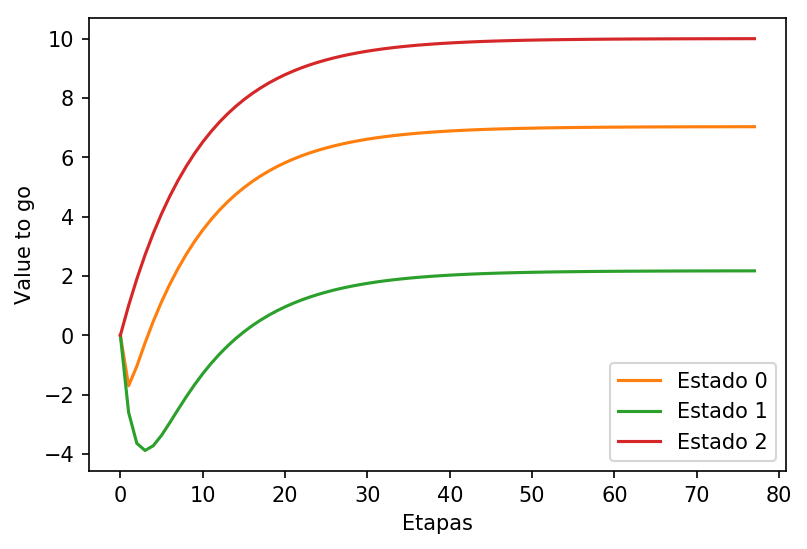
\includegraphics[width=0.5\textwidth]{graphp32a09}
          \caption{Gráfico que muestra la evolución del \textit{value-to-go} de cada estado en función de la  iteración para $\lambda=0.9$}
          \label{iteration 0.9}
        \end{figure}
        \begin{figure}[h]
          \centering
            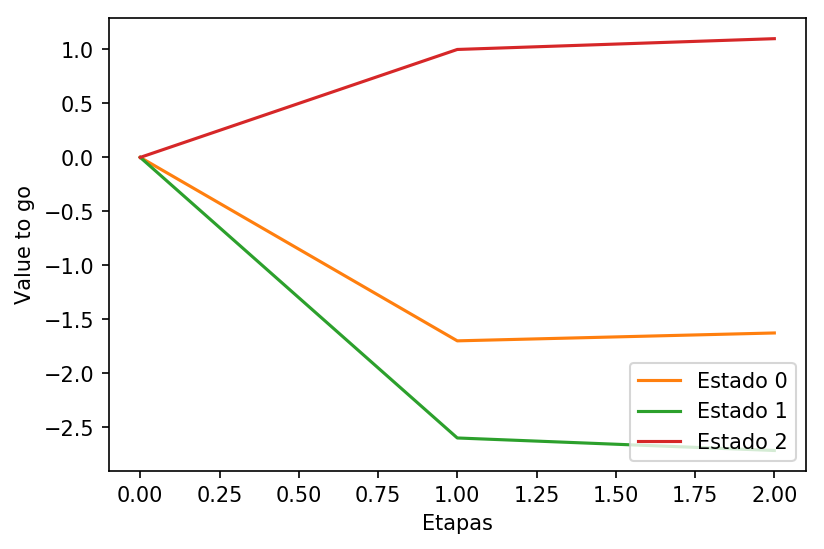
\includegraphics[width=0.5\textwidth]{graphp32a01}
          \caption{Gráfico que muestra la evolución del \textit{value-to-go} de cada estado en función de la  iteración para $\lambda=0.1$}
          \label{iteration 0.1}
        \end{figure}
        
        \item Usando el algortimo de iteración por política para resolver el problema, se tiene que se termina a la primera iteración. Inicia con la política (\textit{azul, verde, gris}) y ya en la segunda iteración llega a su política final (\textit{negro, verde, gris}). Esto es independiente del factor de importancia del futuro. El resultado de la política óptima coincide con el llegado por iteración de valor.
        
        \item 
        
        
        Problema dual
        
        Función objetivo
        $$\max_{f \geq 0} \sum\limits_{s \in \mathds{S}}\sum\limits_{x \in \mathds{X}} r(s,x) \cdot f_{s,x} $$
        
        Restricciones
        $$\sum\limits_{x \in \mathds{X}} f_{s_1,x} - \sum\limits_{s \in \mathds{S}}\sum\limits_{x \in \mathds{X}} \lambda \cdot \mathds{P}(s_1 | s,x) \cdot f_{s,x} = a_{s_1} \quad \forall s_1 \in \mathds{S}$$ \\
        
        Se escoge $a_s = 1 \quad \forall s \in \mathds{S}$ \\
        
        Se llegó a los resultados que se muestran a continuación. Se resolvió en 2 iteraciones, con un valor objetivo óptimo de 19.2069
        \begin{align*}
            f_{0,azul} &= 0 \\
            f_{0,negro} &= 1.0989 \\
            f_{1,verde} &= 2.17391 \\
            f_{1,rojo} &= 0 \\
            f_{2,gris} &= 26.7272 \\
        \end{align*}
        
        Se puede observar que la política óptima corresponde con los $f > 0$. Esta sería entonces (\textit{negro, verde, gris}), igual a la oplítica obtenida cn los métodos de iteración y de valor
      
        
        
    \end{enumerate}
\end{enumerate}

\section{}

\begin{enumerate}
    \item La modelación es la siguiente:
    \begin{itemize}
        \item Etapas: $t \in \{1, \dots, \infty \}$
        \item Estados: $s \in \{0, 1, 2, 3\}$
        \item Decisión: Para cada $s$ existen las siguientes posibles acciones: $$X(s) = \{0, 3 - s\}$$
        \item Probabilidades de transición:
            \[
            p(s_1\mid s, X(s)) =
                 \begin{cases}
                    P(D\geq s+X(s)) \quad \text{si $s_1 = 0$}\\
                    P(D=s+X(s)-s_1) \quad\text{e.o.c}\\
                 \end{cases}
            \]
            Con $s_1 = s+X(s)-d$
        \item Costo inmediato:
            $$r(s, X(s)) = x(s)\cdot h + P(D\geq s + X(s)) \cdot min(0, s+X(s)-D)$$
    \end{itemize}
\end{enumerate}


  

\end{document}